\section{Supplementary Material}
\label{sec:sm}
Section~\ref{subsec:ext_exp} contains extended experiments.
Section~\ref{subsec:usereval} contains our user evaluation questionnaire.
\subsection{Extended Experiments}
\label{subsec:ext_exp}

\begin{figure}[h]
	\centering
	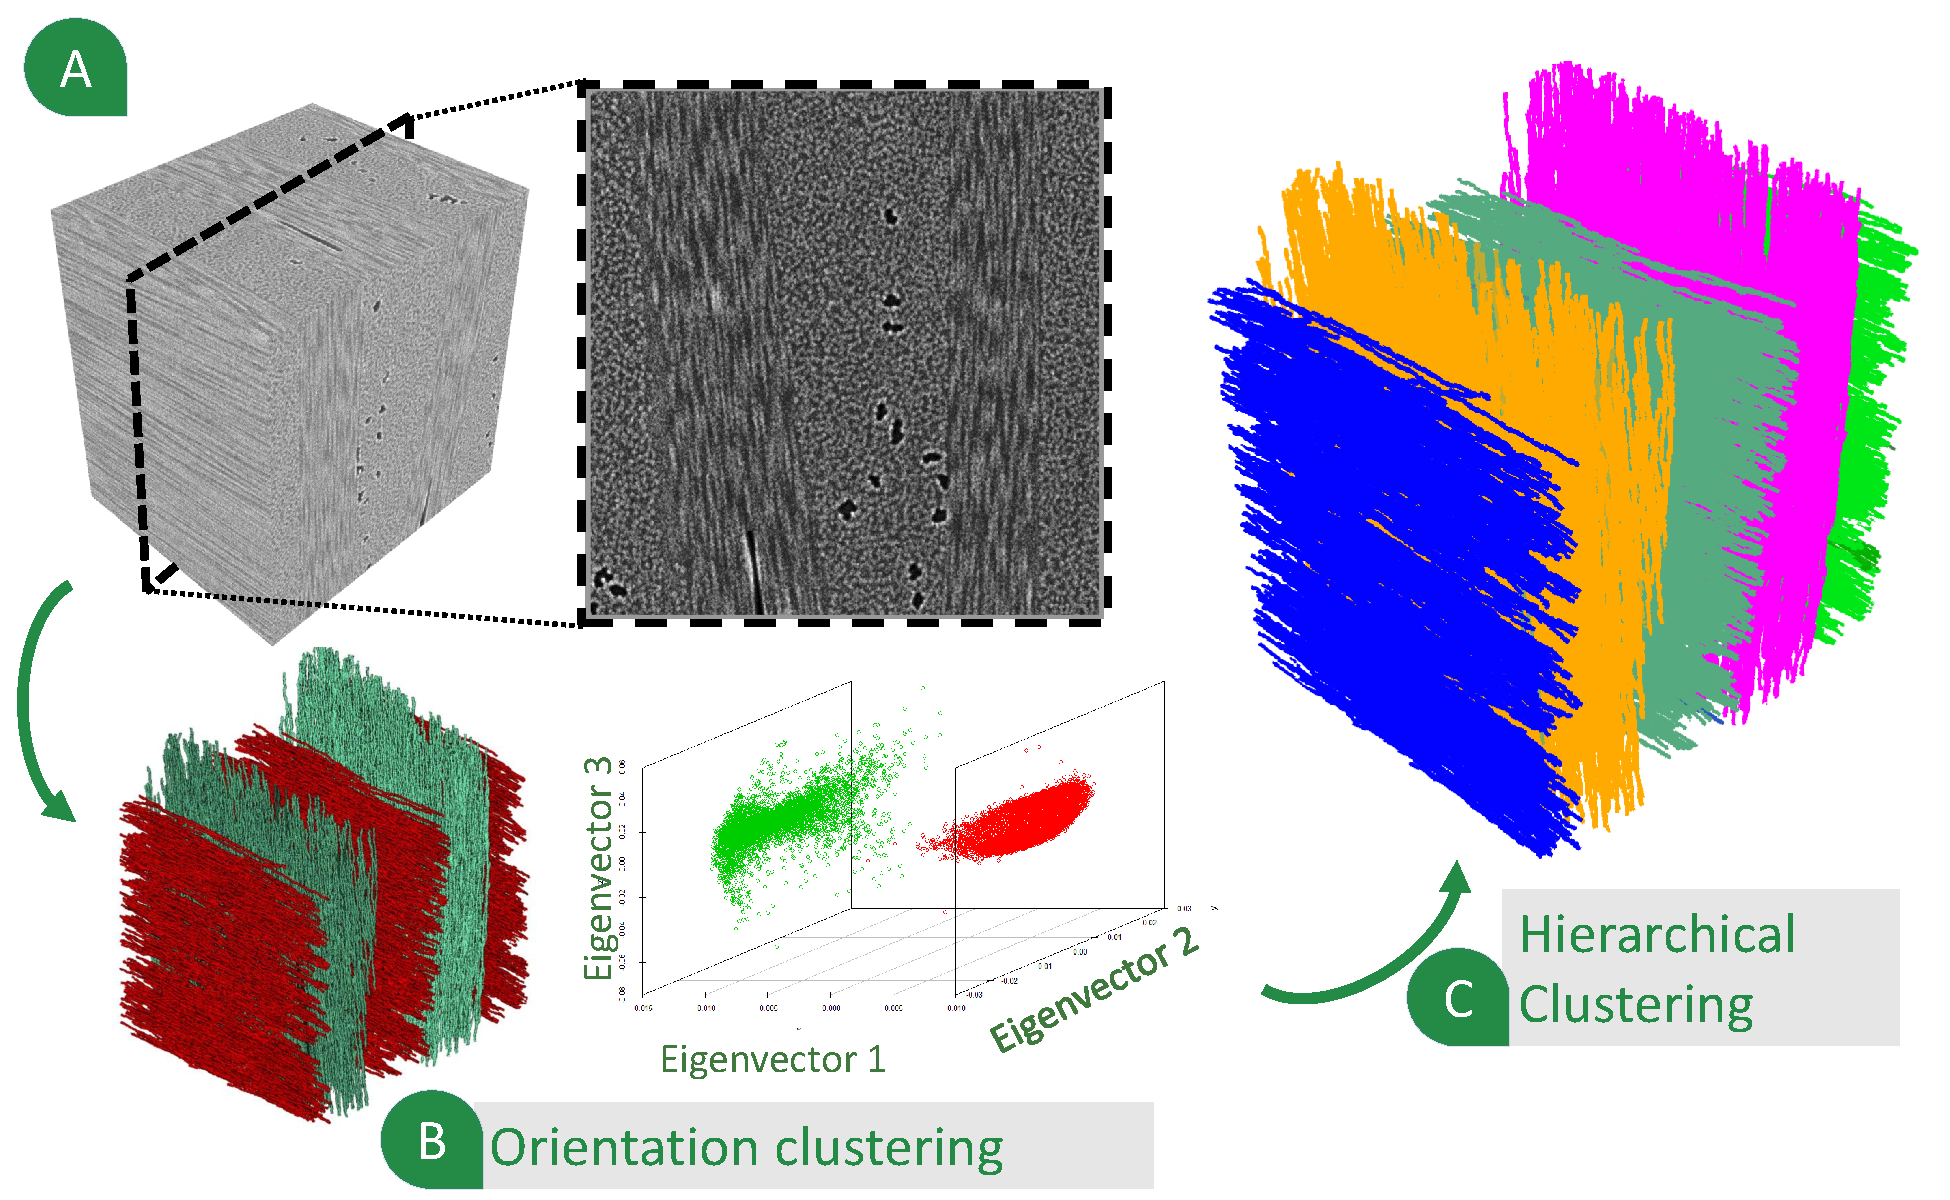
\includegraphics[width=0.7\linewidth]{images_pvis/dataset3.pdf}
	\caption{Results on dataset3. (a) Rendering of our dataset. (b) MetaTracts embedded on the top 3 eigenvectors and clustered into 2 clusters. (c) Each orientation, hierarchically clustered into 10 clusters.}
	\label{fig:dataset3}
\end{figure}
\begin{figure}[h]
	\centering
	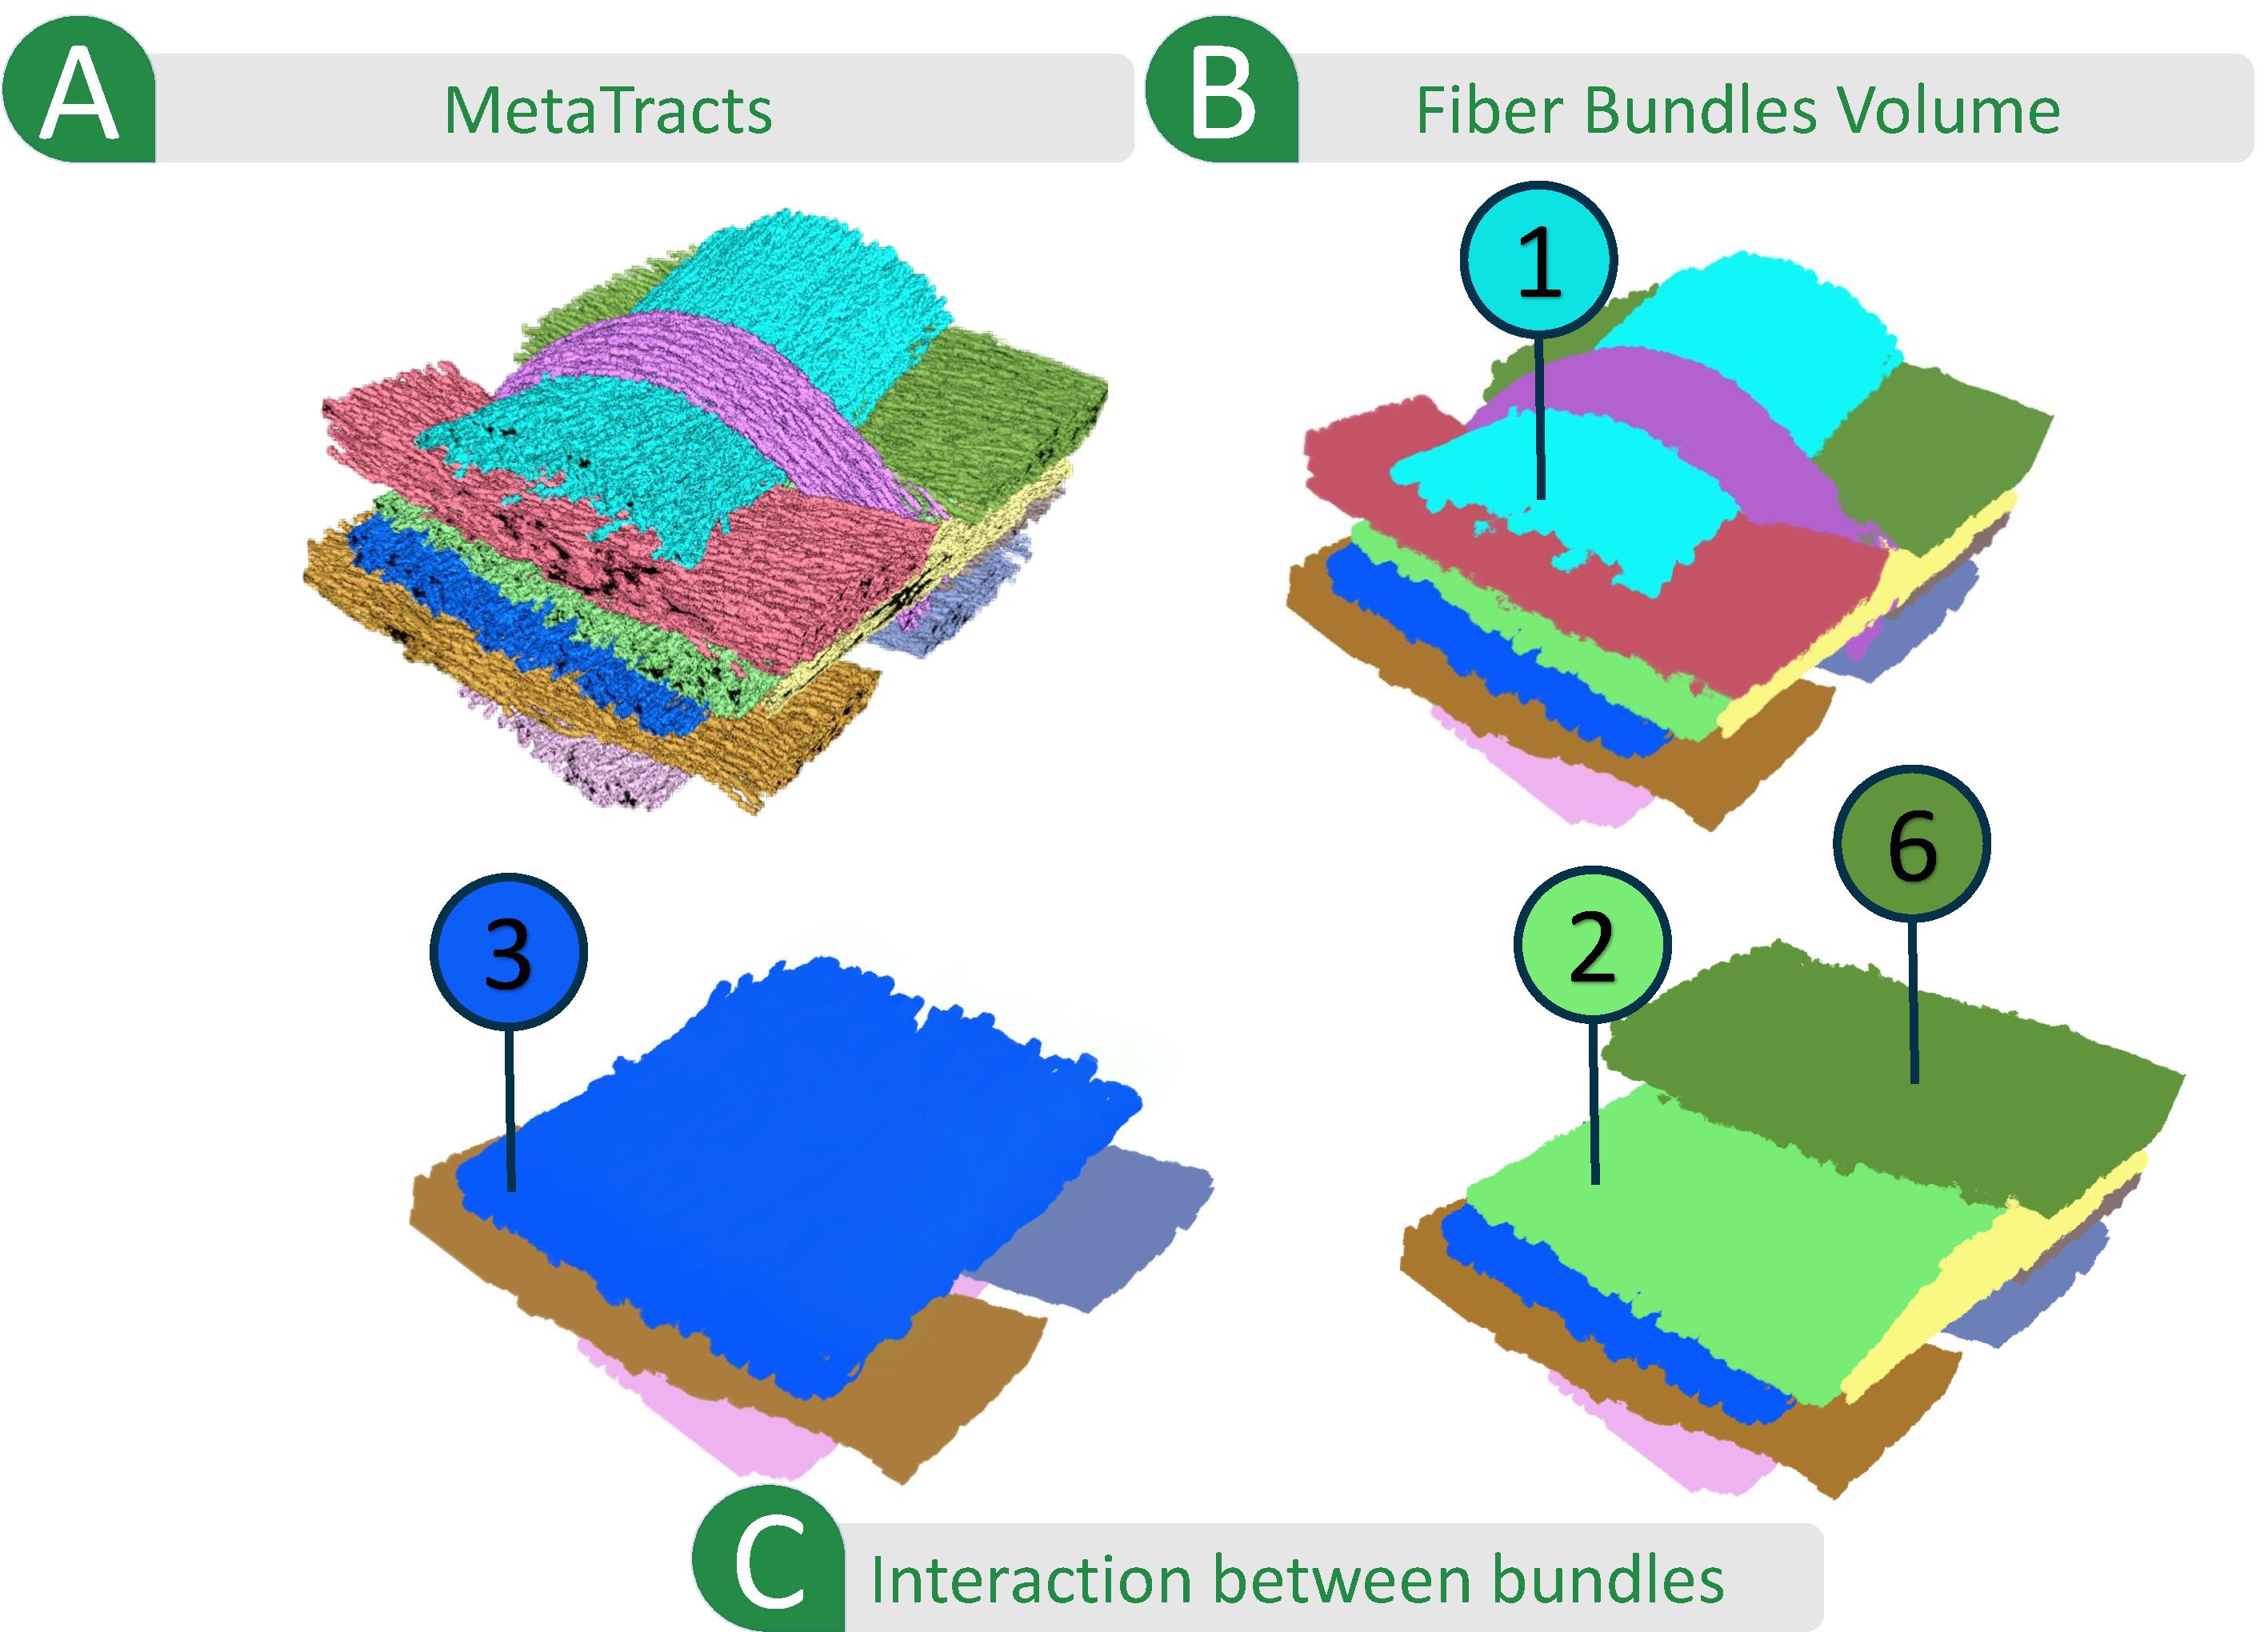
\includegraphics[width=0.7\linewidth]{images_pvis/dataset1-extended.pdf}
	\caption{Results on dataset1. (a) MetaTracts. (b) Voxelized MetaTracts. (c) Subset of the fiber bundles are shown to better visualize the interaction between particular bundles.}
	\label{fig:dataset1-extended}
\end{figure}
Figure~\ref{fig:dataset3} shows the results on our third dataset. The data set is 600$\times$500$\times$600 in size and the datatype is uint16. For testing purposes we have restricted the number of MetaTracts produced to 10000 which generates the empty spaces in Figure~\ref{fig:dataset3}b,c.
The dataset has 5 major bundles. All the bundles were extracted by MetaTracts.

Figure~\ref{fig:dataset1-extended} further shows how spatial context can be used to answer questions such as  Are these bundles in contact at a particular position in the data? What is the relative orientations of the contacting bundles? These bundles are occluded in the original volume and no conclusions can be made from the original volume. In the voxelized MetaTracts we can clearly see where and how the bundles interact.






\subsection{User Evaluation Questionnaire}
The questionnaire contains links to videos which were seen by the participants.
\label{subsec:usereval}
\pagebreak
\includepdf[pages={1-13}]{./supplemental/MetaTracts_usereval.pdf}
